Interaction between human and complex cyber-physical systems is an essential aspect of modern computing platforms. These interactions enable users to provide inputs to software systems and services and interpret computation output. Over the last half a century~\cite{hci_history_1,hci_history_2}, researchers in academia and industry spent a significant effort to make this interaction as effortless as possible. Input-output (IO) peripherals and complex user interfaces (UI) are keys to facilitate this interaction. Such intuitive UIs were quintessential to the widespread deployment of computing devices around us and the rapid adoption of remote applications and services. 

Security and safety-critical remote applications such as e-voting, online banking, industrial control systems (such as remote PLCs~\cite{controlbyweb}), and medical devices~\cite{medicalDevice} rely upon user interaction. This is typically performed through a \emph{host} system that generally is a standard $x86$, which gives the host access to the raw IO data that is exchanged between the user and the remote server. The host consists of large and complex system software such as the operating system, device drivers, applications such as a browser, and a diverse set of hardware components that expose the host to a large attack surface. Due to cost and convenience, general-purpose PCs are prevalent in many safety-critical application domains such as industrial plants and hospitals. For example, the WannaCry ransomware incident showed that NHS hospitals relied on Windows XP platforms~\cite{berry_2017,field_wannacry_2018}. 


\begin{figure}[t]
  \centering
    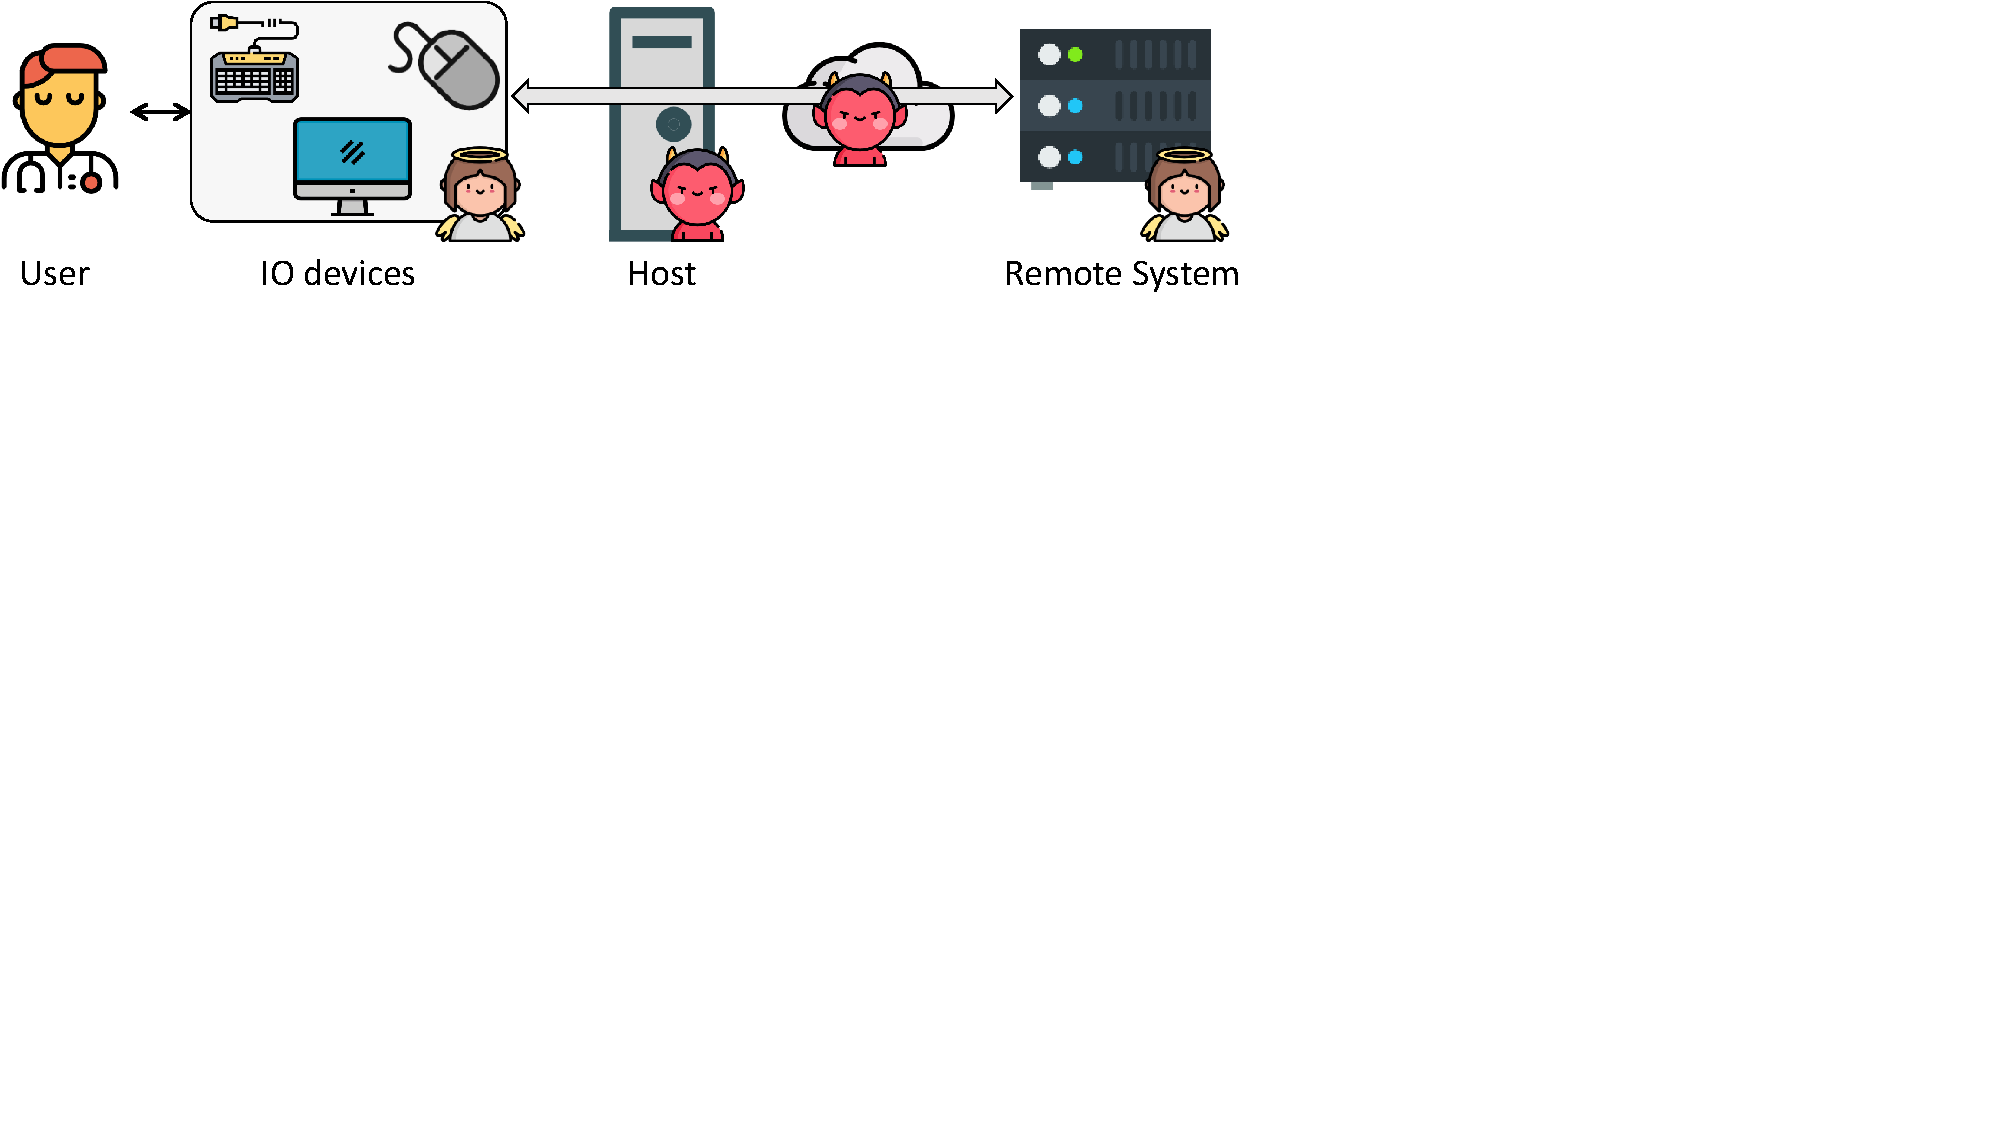
\includegraphics[trim={0 14cm 12cm 0},clip,width=\linewidth]{chapters/introduction/images/trustedPath.pdf}
    \caption[Remote trusted path through untrusted host]{\textbf{Remote trusted path through untrusted host.} The user interacts with a remoter service (that is trusted) with her trusted IO peripherals through the untrusted host and network. A remote trusted path must ensure the integrity (and in some application scenarios, confidentiality) of the data between the user and the remote server.}
    \label{fig:trustedPath}
\end{figure}

\section{Trusted Path}

\emph{Trusted path} provides a secure channel between the user (specifically through the human interface devices - HIDs) and the end-point, typically a trustworthy application running on the host. A trusted path ensures that user inputs reach the intended application unmodified, and all the outputs presented to the user are generated by the legitimate application. In certain scenarios, the trusted path also provides confidentiality of the user data. The trusted path can also be extended to general peripherals such as accelerators, GPUs, and sensors, and even remote systems. An attacker who exploits the software stack, i.e., the hypervisor or the OS and/or the hardware (refer to Figure~\ref{fig:trustedPath}), can control the user's computer. Such an attacker can \emph{observe} and \emph{modify} any user interaction data without being detected by the user or the server, hence undermining the trusted path's properties. 

The trusted path to the local host is a well-researched area where many solutions focus on using trusted software components such as a trusted hypervisor~\cite{zhou2012building} or external trusted hardware~\cite{filyanov2011uni,weigold2011secure,McCPerRei2006,mannan2007using,Fidelius}. However, hypervisors are hard to deploy, have a large TCB, and are impractical in real-world scenarios as most of the existing verified hypervisors offer a minimal set of features, and some of the external device-based approaches suffer from poor usability, security issues due to user habituation and are only limited to simple inputs.


\section{TEEs in Trusted Path}

Trusted execution environments (TEEs) drastically reduce the trusted computing base (TCB) and provide security to applications, known as enclaves, without having to trust the operating system and hypervisor~\cite{costan2016intel,winter2008trusted,costan2016sanctum}. Thus, the attack surface is reduced by eliminating two of the largest sources of vulnerabilities for a system~\cite{checkoway2013iago,suzaki2011memory}. TEEs use isolation primitives provided by the CPU to exclude all software, but a single target application (commonly known as the enclaves) from the software trusted computing base (TCB). Only the CPU is part of the hardware TCB, while the remaining hardware in the system is considered malicious. Even memory is not included in the TCB and can only be used in conjunction with memory encryption and integrity protection. Such a trust model makes the TEEs ideal candidates for the aforementioned trusted path applications where the software stack is attacker-controlled. 


While SGX's remote attestation guarantees that the attested enclave runs the expected code, it \emph{does not}, however, guarantee that the enclave runs on the expected computing platform. An adversary that controls the software stack (OS, hypervisor, etc.) on the target platform can relay incoming attestation requests to another platform. This way, the user ends up attesting to the attacker's platform rather than her own. Relay attack enables the attacker to see all the IO data to and from the user, e.g., sensitive user input on display, and execute a long-term physical side-channel attack. Hence, relay attacks on TEEs pose a real threat to the trusted path. Note that the relay attack is a long-standing open problem in trusted computing, as already a decade ago, Parno identified it in the context of TPM attestation~\cite{parno2008bootstrapping}. Hence, directly incorporating a trusted path to a TEE like Intel SGX is not a trivial issue.


Solving the relay attack still does not make TEEs ideal for a trusted path. TEEs cannot communicate with any external device without going through the malicious operating system, which is crucial for a trusted path. Hence with the current TEEs, the only way to build a trusted path is to rely on the OS or hypervisor with millions of lines of code~\cite{torvalds2020linux,barham2003xen}, results in a static hardware TCB from the enclave's perspective. This shortfall of TEEs is critical because modern, trusted path applications not only handle data for simple IO purposes but also many applications. E.g., using sensitive medical data for training machine learning models on the GPU. This new breed of applications shows a changing trend in cloud computing, known as \emph{disaggregated} computing model. Unlike the traditional CPU-centric computational model, where the CPU is the platform's sole executioner, modern data centers offload application-specific workloads to special-purpose hardware devices such as GPUs, accelerators, etc. Hence the current TEE primitives such as the isolation and the attestation need designing to support the trusted path applications in the modern disaggregated cloud data centers.   